\documentclass[12pt,oneandahalfspaced, a4paper]{tonic-thesis}

%% Some useful LaTeX packages
\usepackage{graphicx}
\usepackage{subfigure}
\usepackage{amsmath}
\usepackage{amsthm}
\usepackage{amsfonts}
\usepackage{amssymb}
\usepackage{cite}
\usepackage{indentfirst}
\usepackage{algorithm}
\usepackage{algorithmic}
\usepackage{array}
\usepackage{booktabs}
\usepackage{tabularx}
\usepackage{rotating}
\usepackage{url}

%% hyperref in PDF
\usepackage{savesym}
\savesymbol{pdfbookmark}
\usepackage{hyperref}
\restoresymbol{HR}{pdfbookmark}
\hypersetup{
    colorlinks,%
    citecolor=black,%
    filecolor=black,%
    linkcolor=black,%
    urlcolor=black,%
    bookmarksnumbered=true
}

\numberwithin{equation}{chapter} %Equation (3.5) instead of Equation (16)

%% Start of your thesis content

\title{Optimization of User Equipment Random Access Delay in LEO Satellite Communication Systems via Synchronization Signal Block Periodicity}
\author{Po-Yu Yen}

\department{Graduate Institute of Communication Engineering}
\degree{Master of Science}
\submitdate{July 2025}
\copyrightyear{2025}

\begin{document}

\begin{preliminary}

\begin{abstract}
% Abstract should advertise the most important results in
% your thesis and the length should be limited to one page.

Low Earth Orbit (LEO) satellite network has been a promising technology due to the wide spread coverage area and high data throughput. However, with the high speed of satellites, frequent handover is unavoidable for user equipments (UEs) on the ground, causing significant interruption time and signaling overhead. Thus, we introduce a quasi-earth-fixed satellite beam scheme to solve the continually handover from the UEs at the cell edge. In this scheme, we allocate the satellite beams to the ground cells in order to maximize overall throughput. After that, we also propose a UE cell selection algorithm, which base on both position information and UE measurement. 
\end{abstract}

\contents

\end{preliminary}


\chapter{Introduction}
\label{chap:introduction}

% Introduction should provide appropriate context and background for your research, such as the recent trend and importance of the technology development related to your thesis.

Non terrestrial network (NTN) has become a promising technique in next generation network. It provides network connectivity to area that traditional network platform cannot reach. For instance, forests, oceans, and deserts. Various platforms are used to provide network services in NTN, such as GEO, MEO, LEO satellites, UAVs, and drones. Among these platforms, LEO satellites are the most actively discussed. These satellites are located at altitude 500 to 2000 kilometers. The strongest advantage is that they provide global coverage, low latency, and high throughput compared to MEO or GEO satellites.

However, to acheive LEO satellite network service, there are some key challanges that need to be resolved. One of the challanges is the unavoidable frequent handover~\cite{38821}. The high speed of LEO satellite forces user equipments (UEs) on the ground to switch the serving satellites frequently, as shown in Figure~\ref{time to ho}. In such scenario, the signalling overhead led by handover signals and the handover interruption time are big issues. 3GPP has discussed some solutions to deal with these issues. By using quasi-earth-fixed cell and satellite switch with re-synchronization~\cite{38300}, the frequent handovers are avoided and the signalling overhead is reduced. For UEs that have already accessed to the network, they can receive the upcoming serving satellite information from the previous one. Also, with the help of the ephemeris data of satellies and the position information of UEs, the matching between satellites and UEs has been largely improved~\cite{38331}. Nontheless, for those UEs who have not access to the network, the random access procedure is the only way for them to get into the network. To establish the connection between satellites and UEs, satellites need to transmit synchronization signal block (SSB) to ground for UEs to capture. Once UEs have successfully receive SSBs, the random access procedure starts and the UEs are able to access to the satellite network. Typically in terrestrial network, ground stations send SSB to the serving area every 20 milliseconds. However, the traditional SSB specifications in LEO satellite communication system do not work because the power budget in LEO satellite is so tight that the power is not enough to send all the serving cells in such a short periodicity. Thus, in this thesis we will find out how to deal with this issue by adjust the SSB periodicity and transmitted power. 

\begin{figure}[h!]
    \centering
    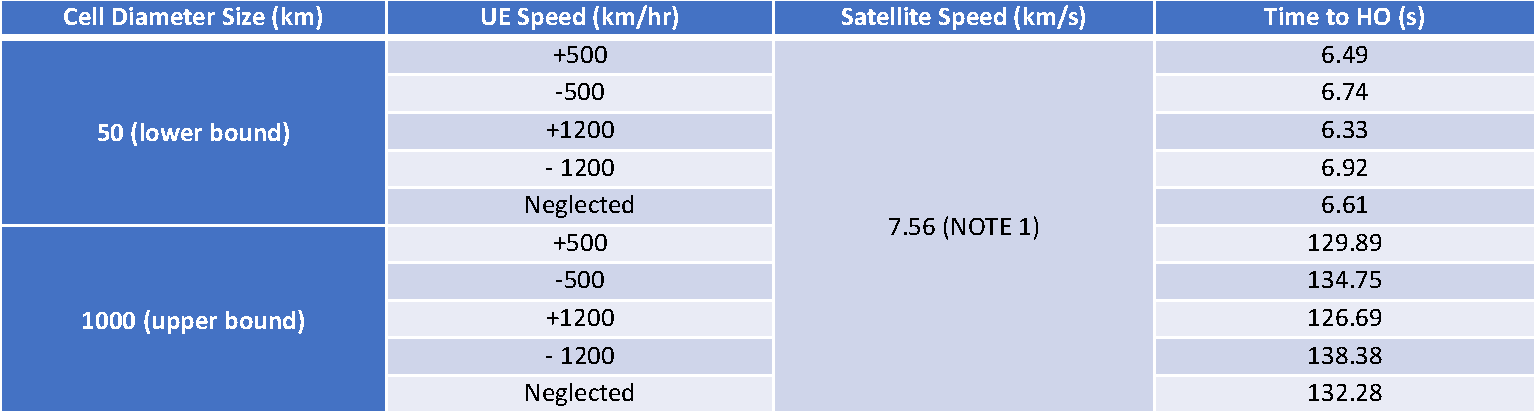
\includegraphics[width=1\textwidth]{figure/time to ho.pdf}
    \caption{Time to handover for min/max cell diameter and varying UE speed}
    \label{time to ho}
\end{figure}
\chapter{Background and Related Work}
\label{chap:background}

% The goal of this chapter is for laying the technical background (such as distributed source coding) for understanding the contribution of your thesis; non-technical background (such as the background of M2M communications) can go to Chapter~\ref{chap:introduction}.

% Related work should be be classified into proper sub-sections depending on the topics
% related to your thesis research.
\section{Random Access Procedure}
The random access procedure in 5G is a critical mechanism that allows a User Equipment (UE) to establish initial uplink synchronization and connect to the network (gNB). The procedure is essential for first-time access, handovers, and re-establishing connections after inactivity or loss of synchronization. Here are some typical steps in contention-based random access: 
\begin{itemize}
    \item Preamble Transmission (Msg1): The UE randomly selects a PRACH (Physical Random Access Channel) preamble and transmits it to the gNB. This "signature" indicates the UE's request for network access.

    \item Random Access Response (Msg2): The gNB detects the preamble and responds with a Random Access Response (RAR), which includes timing adjustment, a temporary identity, and an uplink resource grant. This enables the UE to align its timing with the network and prepare for further communication.

    \item RRC Connection Request (Msg3): Using the granted resources, the UE sends a connection request, which includes its identity and the reason for establishing the connection, such as initial access or handover.

    \item Contention Resolution (Msg4): The gNB sends a contention resolution message confirming which UE has successfully completed the random access. If multiple UEs used the same preamble, only the correct one will be acknowledged, resolving the contention.
\end{itemize}

\section{Synchronization Signal Block}
\subsection{Components of SSB}
The Synchronization Signal Block (SSB) in 5G New Radio (NR) is a critical structure for initial access between the user equipment (UE) and the base station (gNB). Each SSB is composed of three main elements:
\begin{itemize}
    \item Primary Synchronization Signal (PSS): The PSS enables the UE to obtain symbol timing and perform coarse frequency synchronization. It allows the UE to find the starting point of a radio frame and resolves the physical layer cell identity group.
    \item Secondary Synchronization Signal (SSS): The SSS complements PSS by providing additional information to finalize the cell identification and determines the frame timing, which refines synchronization accuracy for the UE.
    \item Physical Broadcast Channel (PBCH): The PBCH conveys essential cell-specific information, including system configuration parameters (such as the System Frame Number), which the UE needs for further connection setup after synchronization.
\end{itemize}
These components jointly allow the UE to perform downlink synchronization, cell identification, and to decode key system information for network access.

\subsection{SSB Configuration}
A series of SSBs called \textit{SSB burst} are sent in a half frame (5ms), the number of SSBs in a SSB burst is determined depends on the carrier frequency and the subcarrier spacing of the transmitted signals. Each cell has a SSB periodicity, defined as the time interval the SSB burst be transmitted to the cell, as shown in Figure~\ref{SSB}. 

\begin{figure}[h!]
    \centering
    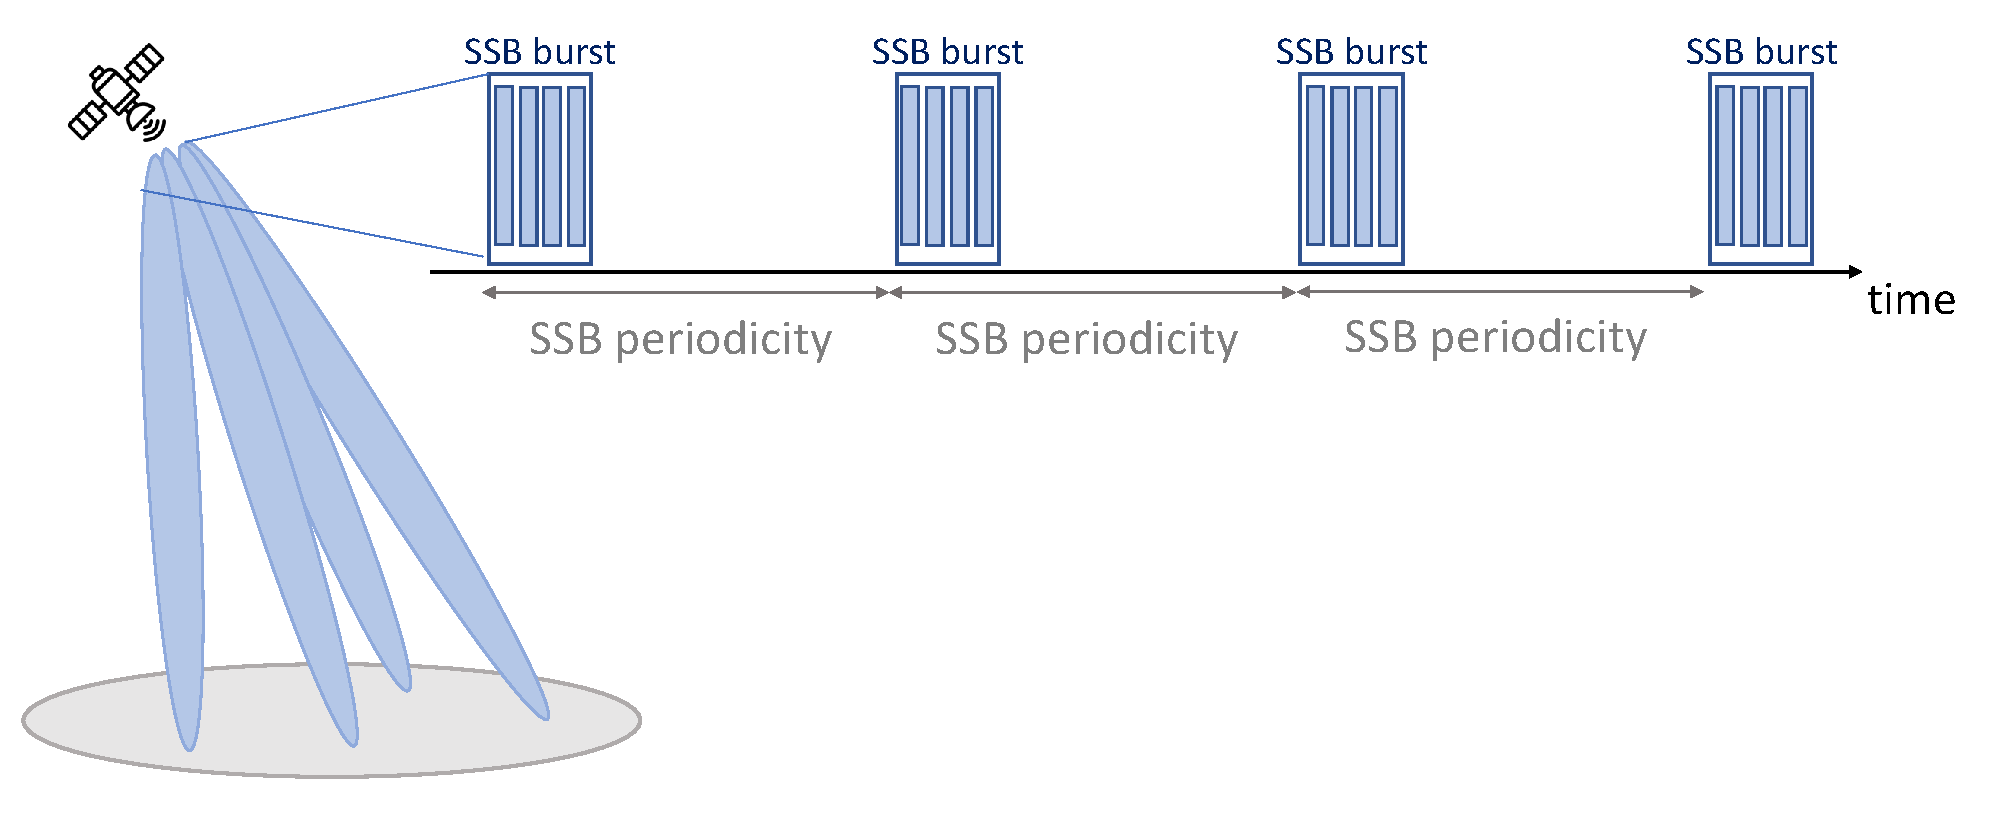
\includegraphics[width=0.8\textwidth]{figure/SSB.pdf}
    \caption{Illustration of SSB configuration.}
    \label{SSB}
\end{figure}

\subsection{SSB in LEO Satellite Network}
In terrestiral network (TN), the base station (gNB) transmits SSBs periodically in time and across different spatial directions through beam sweeping, enabling the UE to detect the best SSB and select the optimal beam for communication. In NTN, the SSBs do the same job but the coverage area of each satellite is much bigger than TN, that means each satellite has to provide service to more cells. Moreover, the long distance from satellite to ground and the power budget of each satellite forces us to properly allocate the power of the SSB. Thus, it is essential for us to manage the SSB transmitted power and the periodicity of each cell.

% The base station (gNB) transmits SSBs periodically in time and across different spatial directions through beam sweeping. Each SSB last for a half frame (5ms). A UE can be provided per serving cell by \emph{ssb-periodicityServingCell}, which is the periodicity of SSB in each serving cell. 

% \subsection{}
% A burst of SSBs covers various directions or beams, enabling the UE to detect the strongest SSB and select the optimal beam for communication. Upon reception, the UE measures the signal quality of the detected SSBs and chooses the best one for initiating the random access procedure.

\section{Related Work}



\chapter{System Model}
\label{chap:model}
% system flow diagram
% satellite orbit pattern
\section{System Overview}

This chapter introduces the LEO satellite communication system, as illustrated in Figure~\ref{fig_system}. We discuss one of the satellites in the LEO satellite communication system. It consists of $M$ beams, represented by $\mathcal{M} = \{m\ |\ m = 1, 2, \ldots, M\}$, and in the coerage area of the satellite it contains $U$ user equipment (UE), indexed by $\mathcal{U} = \{u\ |\ u = 1, 2, \ldots, U\}$.
%TODO: modify to one satellite figure
\begin{figure}[h!]
    \centering
    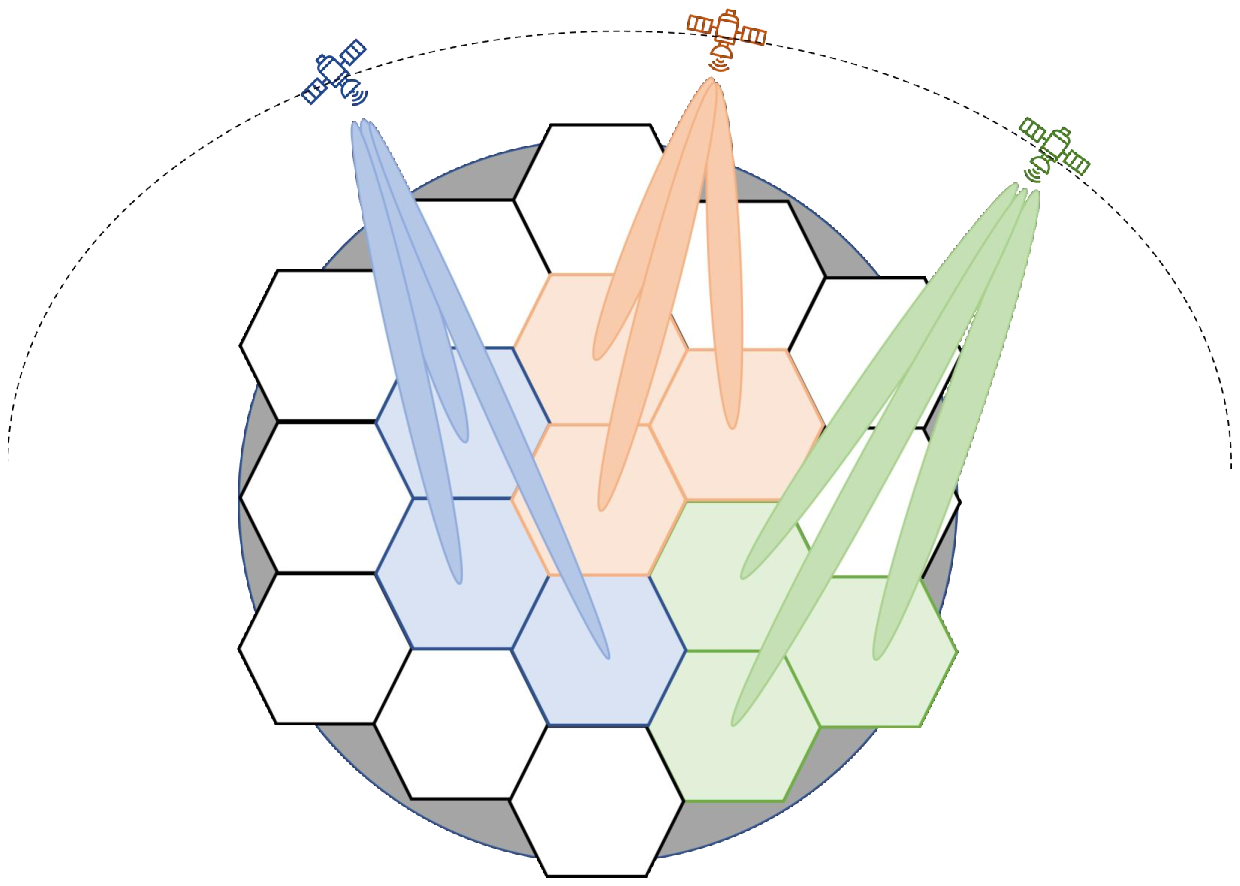
\includegraphics[width=0.8\textwidth]{figure/system overview.pdf}
    \caption{Illustration of satellite beams and cells.}
    \label{fig_system}
\end{figure}

We define a short time $T^{slot}$ as the time duration of a time slot. During one time slot, we assume that the satellite position is fixed, and the SSB periodicity of each cell is fixed.

In this thesis, we adopt the quasi-earth-fixed cell scheme. Unlike the earth-moving cell scheme—where the coverage areas of satellite beams move as the LEO satellites orbit—this approach directs satellite beams so that each beam consistently covers the same geographical cell for a given period. Thus, the coverage area of each satellite beam remains fixed relative to the ground during that interval. Throughout, we assume each satellite beam is oriented toward the center of its designated cell.

We define a power budget for the satellite. Let $P_{m}[t]$ denote the transmitted power of the $m$-th beam from the satellite at time slot $t$. The aggregate transmit power of all beams on the satellite must satisfy:
\begin{equation}
    \sum_{m} P_{m}[t] \leq P_s
\end{equation}
where $P_s$ is the maximum transmit power per satellite.

The locations of UEs wishing to access the network are assigned randomly within their corresponding cells, and the population of each cell are generated according to area population density statistics.

\section{Channel Model}

\subsection{Free Space Path Loss}
In the LEO satellite system, the free space path loss from the satellite to cell $k$ is expressed as follows~\cite{Satellite-Multi-Beam}:
\begin{equation}
    L_{k} = \left(\frac{\lambda}{4\pi d_{k}}\right)^2
\end{equation}
where $\lambda$ is the wavelength, and $d_{k}$ is the distance between the satellite and the center of the $k$-th cell.

\subsection{Shadowed-Rician Fading Channel}
The shadowed-Rician fading model is suitable for satellite communication systems because it accurately reflects the physical propagation environment, capturing both the presence of a strong line-of-sight (LoS) signal and the effects of shadowing from obstacles~\cite{channel-model}. Let $h_{k}$ denote the channel gain between the satellite and the $k$-th cell. The cumulative distribution function (CDF) of the channel gain is:
\begin{equation}
    F_{h_{k}}(x) = K \sum_{n=0}^{\infty} \frac{(m)_n \, \delta^n \, (2b)^{1+n}}{(n!)^2} \, \gamma\left(1+n, \frac{x}{2b}\right)
\end{equation}
where $K = \left(\frac{2bm}{2bm+\Omega}\right)^m/2b$, $\delta = \Omega/(2bm+\Omega)/2b$, $\Omega$ is the average power of the LoS component, $2b$ is the average power of the multipath component except the LoS component, and $m$ is the Nakagami parameter.

\subsection{Antenna Radiation Pattern}
We introduce the antenna radiation pattern in~\cite{Energy-Efficient}:
\begin{equation}
    G(\theta_{m,u}) = G_{max} \left[ \frac{J_1\left(\mu(\theta_{m,u})\right)}{2\mu(\theta_{m,u})}
    + 36 \frac{J_3\left(\mu(\theta_{m,u})\right)}{\mu(\theta_{m,u})^3} \right]^2
\end{equation}
where $\theta_{m,u}$ is the boresight angle between the user position and the beam center with respect to the satellite, $G_{max}$ is the maximum antenna gain, $\mu(\theta)$ is defined as $2.07123 \cdot \sin(\theta)/\sin(\theta_{3dB})$, $\theta_{3dB}$ is the 3 dB half-power beamwidth angle of the antenna, and $J_1(\cdot)$, $J_3(\cdot)$ are the Bessel functions of the first kind of orders 1 and 3, respectively.

With the transmitted power $P_{m}$ from the $m$-th beam of the satellite, the received power at the $u$-th user, $\hat{P}_{m,u}$, is given by:
\begin{equation}
    \hat{P}_{m,u} = P_{m} \cdot L_{k} \cdot h_{k} \cdot G(\theta_{m,u})
\end{equation}
where $k$ is the cell where user $u$ is located.

\section{Synchronization Signal Block Model}

%TODO T^SSB_m vs T^SSB_k
This section describes the SSB periodicity settings and their impact on system operation based on 3GPP protocol. We denote the SSB periodicity of a beam $m$ as $T^{SSB}_m$. The number of SSB in each SSB burst is $B$. Then for each time slot, a beam can serve $T^{slot} \cdot B / T^{SSB}_m$ cells in its coverage area.

\section{Ground Cell Model}

To achieve optimal coverage and minimize overlap, all ground cells are arranged in a regular hexagonal grid, ensuring uniform cell size, as shown in Figure~\ref{fig_system}. Each cell is served by at most one satellite beam in each time slot. To optimize the network coverage, we adjust the size of each cell. The larger cell size decreases the number of cells one satellite has to serve, but the power requirement for a beam to cover a cell increases. On the other hand, if a smaller cell is used, the UEs are able to receive the beam with more precise angle. Nonetheless the number of cells is large for the serving satellite to handle. Thus, we define the area of each ground cell as $A^{cell}$, and the serving area of the satellite as $A^{total}$. The number of cells the satellite serves is then calculated as $K = \frac{A^{total}}{A^{cell}}$, denoted as $\mathcal{K} = \{k\ |\ k = 1, 2, \ldots, K\}$.
%TODO: K is not equal to A^total / A^cell

\section{UE Random Access Delay}
The random access delay $T_u$ for the $u$-th UE is a random variable, defined as the time duration between the start of SSB measurement and the successful reception of SSB, as shown in Figure~\ref{RAD}. $T_u$ can be decomposed into two parts: $T_u^i$ (initial waiting time) and $T_u^l$ (additional delay due to failed attempts). $T_u^i$ is a random variable that represents the time from the start of SSB measurement to the arrival of the first SSB, and $T_u^l$ is another random variable that represents the time from the first SSB arrival to the successful SSB reception.

%TODO: k_u definition
Since the UE can start SSB measurement at any time, $T_u^i$ is a uniformly distributed random variable $U(0, T_{k_u}^{SSB})$. $T_u^l$ is a multiple of $T_{k_u}^{SSB}$, depending on the number of failures $Q_u$. If the received SSB power $\hat{P}_{m, u}$ is less than the threshold $P^{th}$, the UE fails to measure SSB. The probability that the received SSB power is less than $P^{th}$ is denoted as $R_u$. The mathematical formulation is as follows:
\begin{equation}
    T_u = T_u^i + T_u^l
\end{equation}
\begin{equation}
    F_{T_u^i}(t) =
    \begin{cases}
        \frac{t}{T_{k_u}^{SSB}}, & 0 \leq t < T_{k_u}^{SSB} \\
        1, & t \geq T_{k_u}^{SSB} \\
        0, & \text{otherwise}
    \end{cases}
\end{equation}
\begin{equation}
    T_u^l = Q_u \cdot T_{k_u}^{SSB}
\end{equation}
\begin{equation}
    \Pr\left[Q_u = n\right] = (1 - R_u) (R_u)^n
\end{equation}
where $k_u$ is the cell where the $u$-th UE is located, and $F_{T_u^i}(t)$ is the CDF of $T_u^i$.

\begin{figure}[h!]
    \centering
    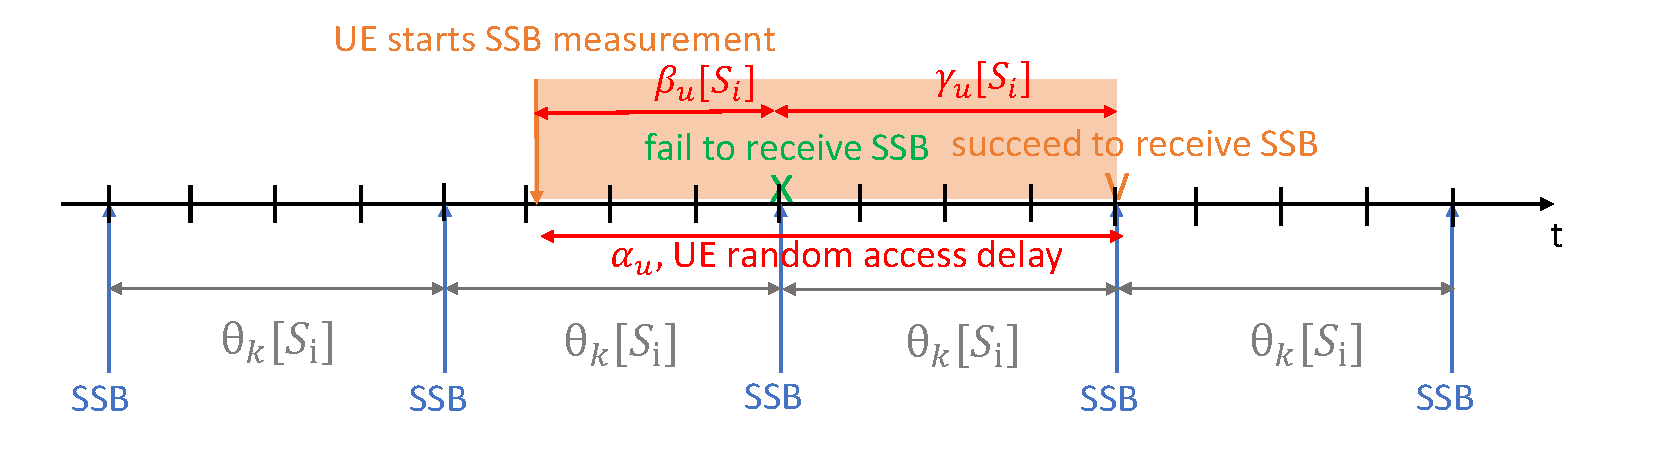
\includegraphics[width=1\textwidth]{figure/random access delay.pdf}
    \caption{Illustration of UE random access delay. $T_u$ is decomposed into $T_u^i$ (initial waiting time) and $T_u^l$ (additional delay due to failed attempts).}
    \label{RAD}
\end{figure}
% TODO: time slot vs. time instant, some variables have t and some don't

\section{Problem Formulation}
This section formulates the optimization problem based on recent 3GPP standardization discussions. In the 3GPP RAN1 \#116 meeting~\cite{ran1-116}, further specifications for the LEO satellite communication scenario were defined. The main challenge is to provide random access to a large number of cells with limited satellite power. Extending the SSB periodicity for some cells reduces satellite power consumption but increases UE random access delay. The transmitted SSB power also affects the success probability of the random access procedure. The trade-off among power allocation, SSB periodicity, and UE random access delay is modeled as follows:
% TODO: mathematical calculation on cdf of Qu
% TODO: reduce satellite power consumption???
\begin{equation}
\begin{aligned}
    & \underset{\Delta, P_{n, m}}{\text{min}} \sum_{u \in \mathcal{U}} T_u \\
    & \text{subject to} \\
    & \quad \sum_{m} P_{n,m}[t] \leq P_s, \quad \forall n \in \mathcal{N} \\
    & \quad |\Delta_{n, m}[t]| \in \{0, 1, 2, 4, 8\}, \quad \forall n \in \mathcal{N}, m \in \mathcal{M} \\
    & \quad \Delta_{n, m}[t] \cap \Delta_{n', m'}[t] = \emptyset, \quad \forall n, n' \in \mathcal{N}, m, m' \in \mathcal{M}, (n, m) \neq (n', m')
\end{aligned}
\end{equation}

% \section{List of Symbols}
% \begin{tabular}{ll}
% \hline
% \multicolumn{2}{l}{\textbf{Symbol}} \\
% \hline
% $N$ & Number of satellites \\
% $M$ & Number of beams per satellite \\
% $K$ & Number of cells on the ground \\
% $U$ & Number of user equipments (UEs) \\
% $L_{n,k}$ & Free space path loss from satellite $n$ to cell $k$ \\
% $h_{n,k}$ & Channel gain between satellite $n$ and cell $k$ \\
% $G(\theta_{n,m,u})$ & Antenna gain for user $u$ \\
% $T^{SSB}_k$ & SSB periodicity of cell $k$ \\
% $T_u$ & Random access delay of UE $u$ \\
% $P_{n,m}$ & Transmitted power of satellite $n$'s $m$-th beam \\
% $P_s$ & Maximum transmitted power for each satellite \\
% $P_{th}$ & SSB reception threshold \\
% $Q_u$ & Number of failed SSB attempts for UE $u$ \\
% \end{tabular}
\chapter{Proposed Algorithm}
\label{chap:algorithm}
Alternating optimization is a widely used strategy for non-convex problems that involve multiple variables or mixed types of parameters. The core idea is to decompose the original challenging joint optimization into two or more easier subproblems, which are solved iteratively. In our problem, we first fix the power allocation $P$ and optimize the SSB periodicity $\theta$. Then, we fix the SSB periodicity $\theta$ and optimize the power allocation $P$. This process repeats until convergence. Thus, the problem (\ref{eq:main}) can be devided to two subproblems. 

\section{Fix Power Optimize SSB Periodicity}

\begin{subequations} \label{eq:FPOS}
\begin{align}
    &\min_{\theta} \sum_{u} \sum_{s\in S} \mathbb{E}[\alpha_u[s]] \\ 
    &\text{subject to} \nonumber \\
    &\theta_k[\mathcal{S}_i] \leq N, \quad \forall k\in\mathcal{K}, \mathcal{S}_i\in\mathcal{\widetilde{S}} \\
    &\theta_k[\mathcal{S}_i] \in \mathbb{N}^+, \quad \forall k\in\mathcal{K}, \mathcal{S}_i\in\mathcal{\widetilde{S}} \\
    &\sum_k \frac{1}{\theta_k[\mathcal{S}_i]} \leq M, \quad \forall \mathcal{S}_i\in\mathcal{\widetilde{S}}
\end{align}
\end{subequations}

\begin{algorithm}[H]
    \caption{Fix Power, Optimize SSB Periodicity}
    \label{alg:FPOS}
    \begin{algorithmic}[1]
        \REQUIRE{}
        Given the transmission power $P_{k, \mathcal{S}_i}$ for each cell $k$ at each epoch $\mathcal{S}_i$, as well as the user distribution.
        \ENSURE
        Find and assign the optimal SSB periodicity $\theta_{k,\mathcal{S}_i}$for each cell, such that the user access delay is minimized while the periodicity configuration for all cells meets the available resource constraints.
        \FOR{every epoch $\mathcal{S}_i$}
        \STATE initialize the SSB periodicity $\theta_{k,\mathcal{S}_i}$ for all cells $k$. 
        \STATE Compute the expected random access delay $\mathbb{E}[\alpha_u[s]]$ for each UE. 
        \STATE According to the periodicity formulas (3.7~3.11), combine transmission power, path loss, and antenna gain to calculate the success probability of SSB reception for each cell.
        \STATE Continuously adjust $\theta_{k,\mathcal{S}_i}$ such that the delay and the resource constraint are satisfied.
        \STATE Finally, obtain the periodicity allocation that yields the minimum delay.
        \ENDFOR
    \end{algorithmic}
\end{algorithm}

\section{Fix SSB Periodicity Optimize Power}

\begin{subequations} \label{eq:main}
\begin{align}
    &\min_{P} \sum_{u} \sum_{s\in S} \mathbb{E}[\alpha_u[s]] \\ 
    &\text{subject to} \nonumber \\
    &\sum_{m} \frac{P_{k}[\mathcal{S}_i]}{\theta_k[\mathcal{S}_i]} \leq P^{total}, \quad \forall \mathcal{S}_i \in \mathcal{\widetilde{S}}  \\ 
    &P_k[\mathcal{S}_i]\geq 0, \quad \forall k\in\mathcal{K}, \mathcal{S}_i\in\mathcal{\widetilde{S}}
\end{align}
\end{subequations}

\begin{algorithm}[H]
    \caption{Fix SSB Periodicity, Optimize Power}
    \label{alg:FSOP}
    \begin{algorithmic}[1]
        \REQUIRE{}
        Given the transmission power $\theta_{k,\mathcal{S}_i}$ for each cell $k$ at each epoch $\mathcal{S}_i$, as well as the user distribution.
        \ENSURE
        Find and assign the optimal SSB periodicity $P_{k, \mathcal{S}_i}$ for each cell, such that the user access delay is minimized while the periodicity configuration for all cells meets the available resource constraints.
        \FOR{every epoch $\mathcal{S}_i$}
        \STATE initialize the transmit power $P_{k, \mathcal{S}_i}$ for all cells $k$. 
        \STATE Compute the expected random access delay $\mathbb{E}[\alpha_u[s]]$ for each UE. 
        \STATE According to the periodicity formulas (3.7~3.11), combine transmission power, path loss, and antenna gain to calculate the success probability of SSB reception for each cell.
        \STATE Continuously adjust $P_{k, \mathcal{S}_i}$ such that the delay and the resource constraint are satisfied.
        \STATE Finally, obtain the power allocation that yields the minimum delay.
        \ENDFOR
    \end{algorithmic}
\end{algorithm}


% \begin{algorithm}[H]
% \caption{Resource Re-balancing Algorithm}
% \label{alg:rebalancing_algorithm}
% \begin{algorithmic}[1]
% \REQUIRE{}

% Total available resources $M_{total}$ (a positive integer representing the total resources),

% Set of groups $\{G_l \mid l = 1, 2, \dots, |\textbf{G}|\}$ (where $|\textbf{G}|$ is the total number of groups),

% For each group $l = 1$ to $|\textbf{G}|$, the estimated number of users $|G_l|^{(t)}$ at time $t$ (a non-negative integer),

% Collision rate model $P_{Collision}^{G_l}(R)$ for each group $l$ (a function that computes collision rate given allocated resources $R$),

% Minimum acceptable collision rate threshold $\epsilon$ (a real number, $0 < \epsilon < 1$).


% \ENSURE
% Optimal resource allocation vector $\{ M_{l} \}_{l=1}^{|\textbf{G}|}$

% \STATE \COMMENT{\textbf{Phase I: Demand calculation and judgment}}
% \FOR{$l = 1$ to $|\textbf{G}|$}
% \STATE Calculate minimum resource requirement $M_{l}^{\min}$ to meet $P_{Collision}^{G_{l}} < \epsilon$
% \ENDFOR
% \STATE $M_{\mathrm{sum}} \gets \sum_{l=1}^{|\textbf{G}|} M_{l}^{\min}$

% \IF{$M_{\mathrm{sum}} \le M_{total}$}
% \STATE $M_{l} \gets M_{l}^{\min}$ for all $l$ \COMMENT{Resources are sufficient, direct allocation}
% \STATE $M_{\mathrm{remaining}} \gets M_{total} - M_{\mathrm{sum}}$
% \STATE $\text{quotient} \gets \lfloor M_{\mathrm{remaining}} / |\textbf{G}| \rfloor$ \COMMENT{Resources per group}
% \STATE $\text{remainder} \gets M_{\mathrm{remaining}} \bmod |\textbf{G}|$ \COMMENT{Remaining resources}
% \FOR{$l = 1$ to $|\textbf{G}|$}
% \STATE $M_{l} \gets M_{l} + \text{quotient}$ \COMMENT{Add base allocation to each group}
% \IF{$l \le \text{remainder}$}
% \STATE $M_{l} \gets M_{l} + 1$ \COMMENT{Add one extra resource to first 'remainder' groups}
% \ENDIF
% \ENDFOR
% \STATE \textbf{return} $\{M_{l}\}$
% \ENDIF

% \STATE \COMMENT{\textbf{Phase II: Resource rebalancing (resource shortage)}}
% \STATE $w_l \gets |G_l|^{(t)} / \sum_{i=1}^{|\textbf{G}|} |G_i|^{(t)}$ for all $l$ \COMMENT{Calculate weight}
% \FOR{$l = 1$ to $|\textbf{G}|$}
% \STATE $M_{l} = w_l \cdot M_{total}$ \COMMENT{Resources allocation based on weight}
% \ENDFOR

% \STATE \textbf{return} $\{M_{l}\}$
% \end{algorithmic}
% \end{algorithm}




\chapter{Performance Evaluation}
\label{chap:results}

All figures should be of the same width whenever possible for consistency.

\section{Simulation Setup}

We use BONMON~\cite{bonmin} to solve the optimization problem.
The simulation setup follows that in~\cite{TR37-868}.

\section{Simulation Results}


\chapter{Conclusion and Future Work}
\label{chap:conclusion}





\begin{postliminary}

\bibfiles{reference}
\bibliographystyle{IEEEtran}

\references

\end{postliminary}


\end{document}
